\section{Assumptions}

This thesis posits that high-level musical concepts manifest over time and remain invariant to specific attributes such as tonal quality, tempo, key, orchestration, signal noise, etc. This is akin to a sheet music composition performed in myriad ways using diverse instruments and styles while preserving its essence.

Abstract features, such as melody, harmony, rhythm, tempo, form, and expression, can be identified irrespective of waveform or production style. This approach offers an objective and comprehensive insight into a piece's musical content and meaning, analogous to how analyzing sheet music unveils a composition's underlying structure and intent.

Although a waveform might have limited sheet music representations that accurately encapsulate its musical components, a single sheet music composition can be performed infinitely using various instruments, voices, tempos, and interpretations. The distinct tonal quality of a waveform is significantly influenced by the specific instrument timbre or production technology employed in its creation, complicating the transcription of its sonic properties into precise sheet music notation.

Moreover, this distinct tonal quality is represented by high-level natural language concepts embedded within a rich cultural and sociological tradition.


\begin{figure}
    \centering
    \scalebox{0.9}{
    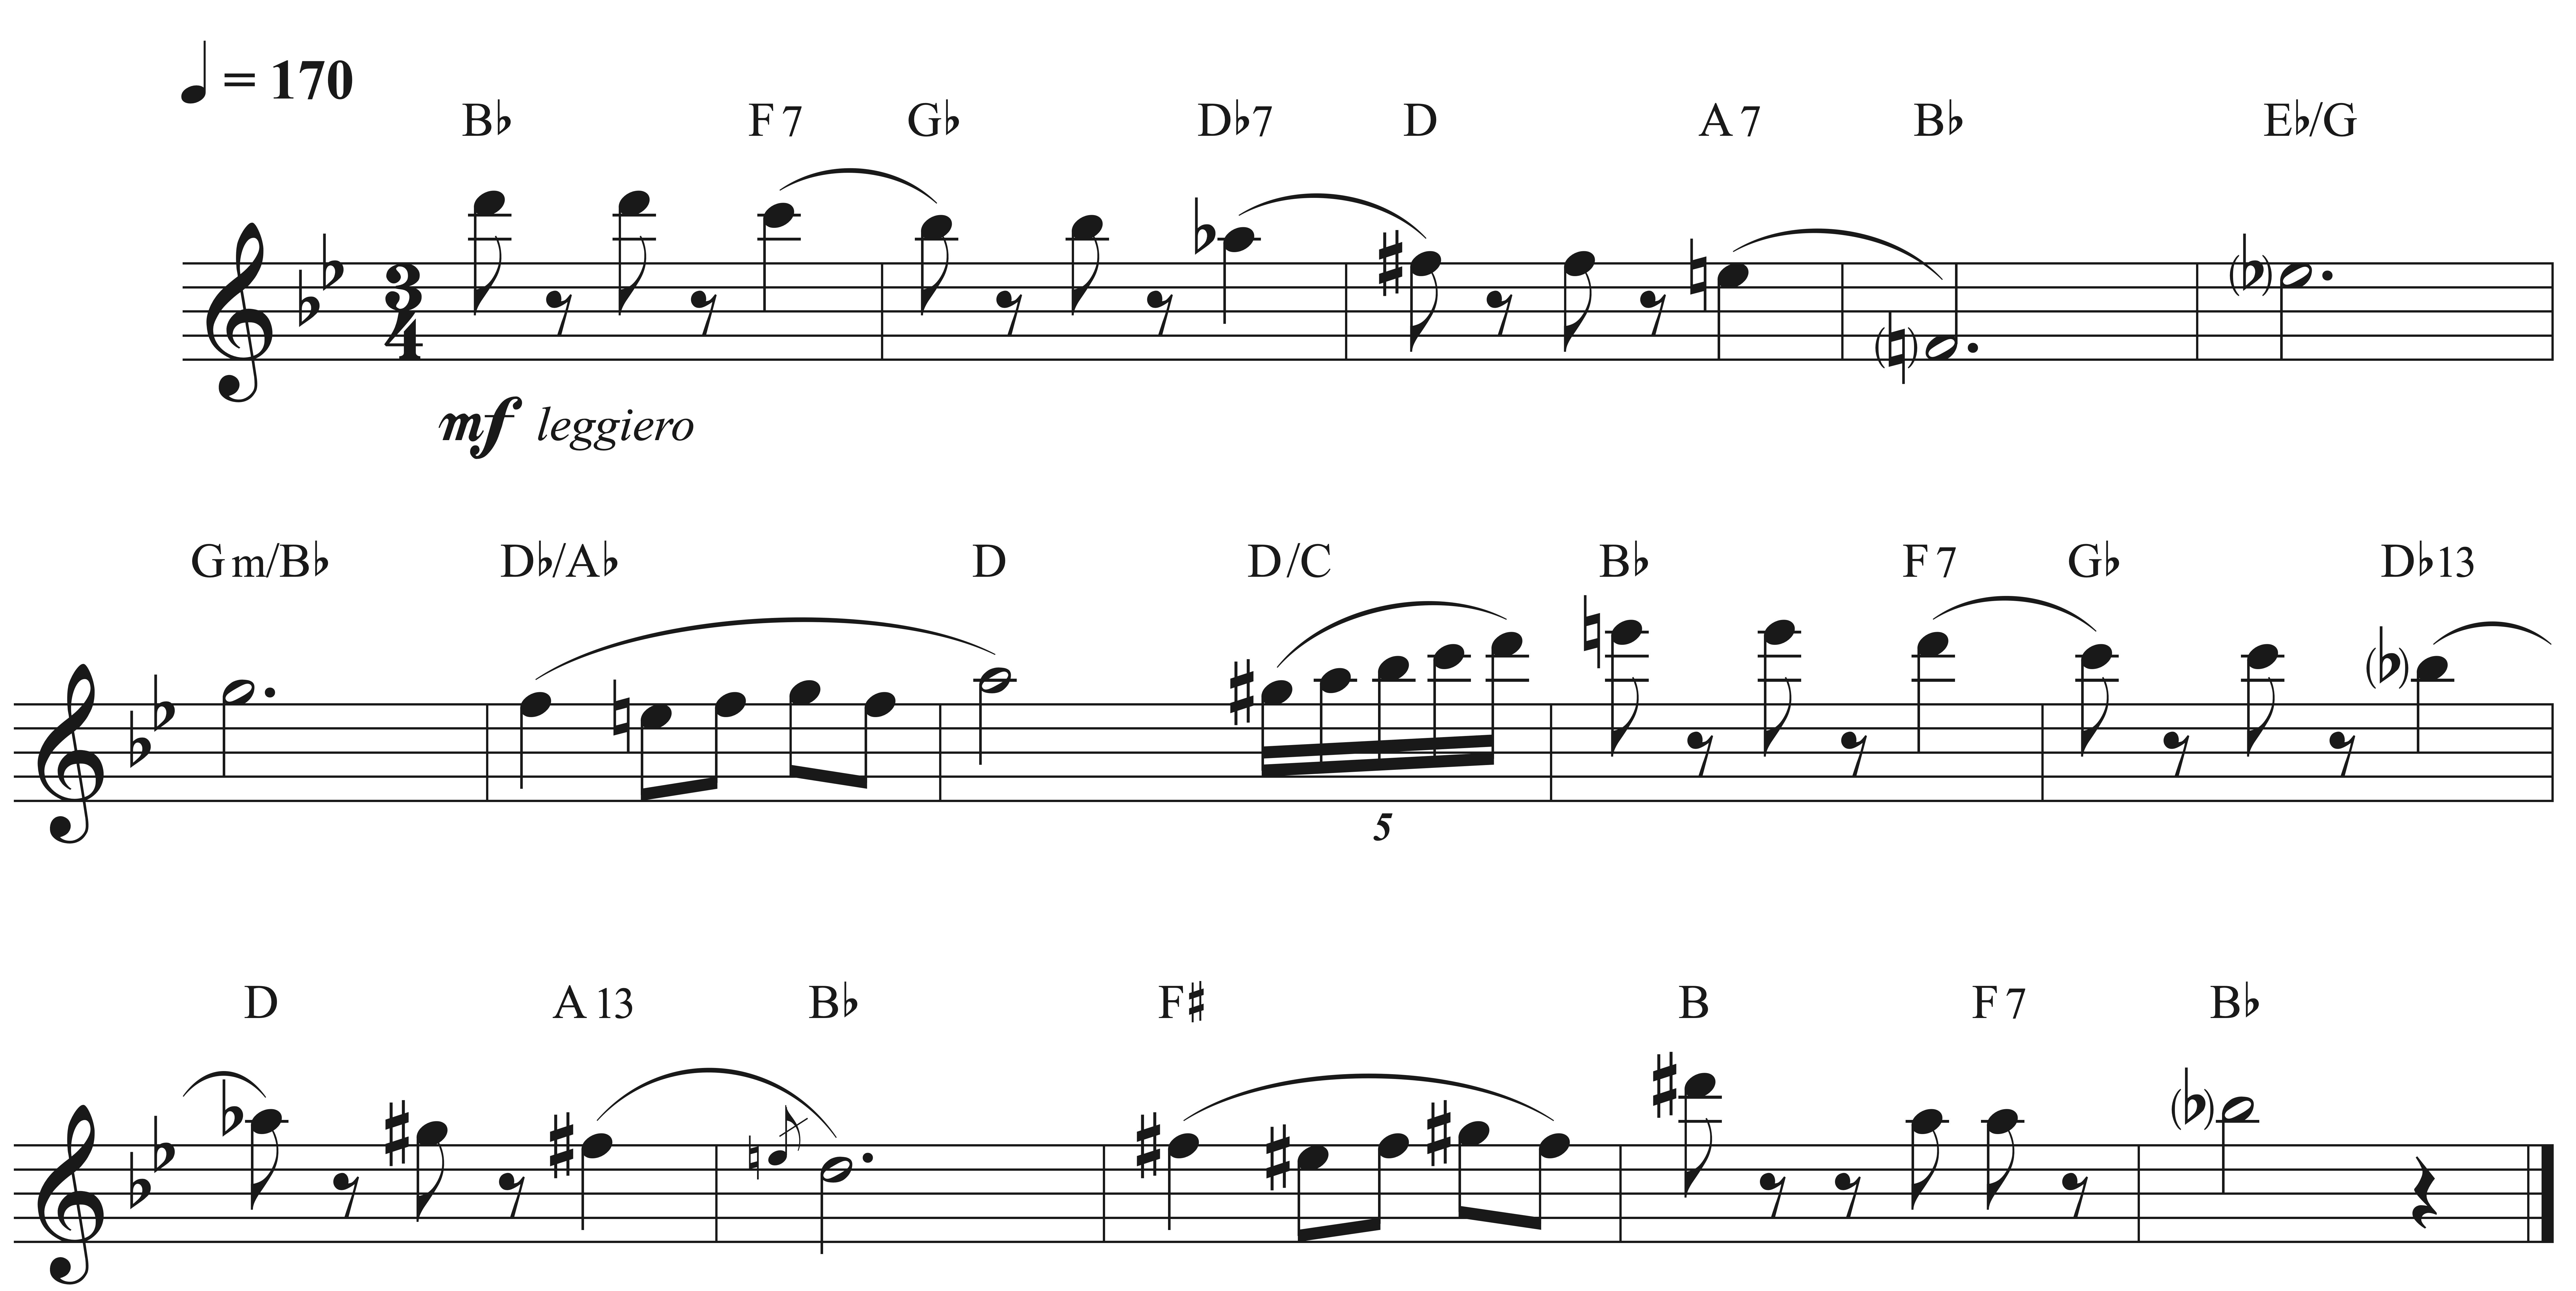
\includegraphics[width=\textwidth]{figures/images/Mahler 9 Giant Steps score.png}
        }
    \caption[Mahler's 9th Symphony, 2nd movement]{\small{A small excerpt from Mahler's 9th Symphony, 2nd movement: The melodic and harmonic contour propels through non-diatonic major thirds.}}
    \label{fig:mahler}
\end{figure}

\begin{figure}
    \centering
    \scalebox{0.9}{
    \includegraphics[width=\textwidth]{figures/images/giant steps score.png}
        }
    \caption[Giant Steps]{\small{John Coltrane's Giant Steps head: A testament to harmonic exploration, featuring rapid chord changes in non-diatonic major thirds.}}
    \label{fig:giant_steps}
\end{figure}

\begin{figure}
    \centering
    \scalebox{0.9}{
    \includegraphics[width=\textwidth]{figures/images/train interlude score.png}
        }
    \caption[Last Train Home]{\small{Pat Metheny's Last Train Home interlude.}}
    \label{fig:last_train}
\end{figure}


\subsection{Beyond Digital Signal Processing (DSP)}

We argue that MIR research needs to incorporate a more balanced approach that considers the interdisciplinary nature of music and the importance of other domains beyond DSP.